\documentclass{article}
\usepackage{graphicx}
\usepackage{hyperref}
\begin{document}

\begin{figure}
    \centering
    \caption{\label{fig:thename}AIT Brainlab Logo}
    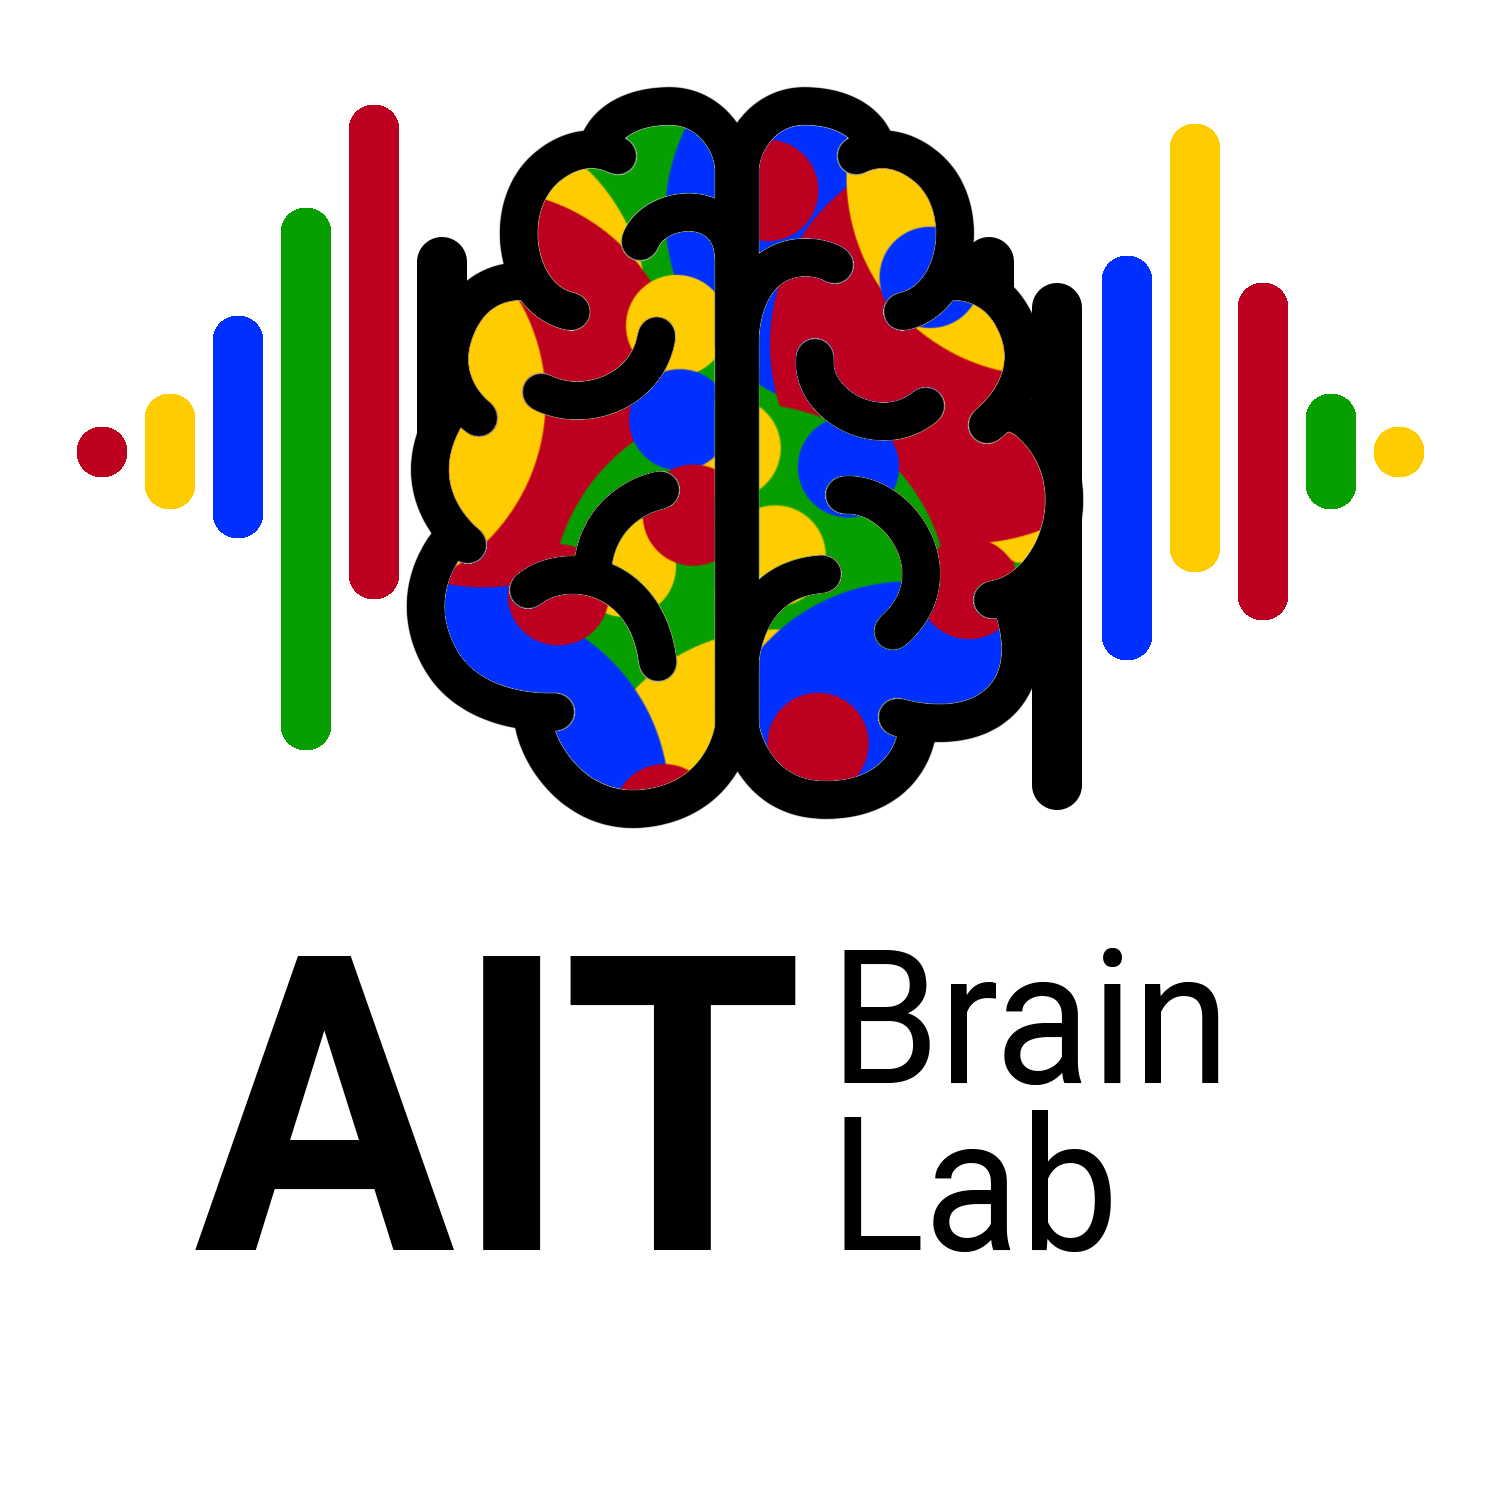
\includegraphics[width=0.75\textwidth]{figures/bci-logo.png}
\end{figure}

figure \ref{fig:thename}

\newpage

There are two ways to write math equation.

Inline equation $y = ax + b$ is a linear equation

Display equation $$ y = ax + b $$ is a linear equation.

\begin{enumerate}
    \item $y = ax + b$
    \item ** \( y = ax + b \)
    \item \begin{math}
        y = ax + b
    \end{math}
\end{enumerate}

1. 
$$ y = ax + b $$

2.
\[ y = ax + b \]

3. 
\begin{displaymath}
    y = ax + b
\end{displaymath}

4. 
\begin{equation}
    y = ax + b
    \label{equ:linear}
\end{equation}

$$ 
 x^{2}_{1}
$$

Refer to this equation~\ref{equ:linear}

\newpage




\end{document}